\documentclass[journal]{IEEEtran/IEEEtran}
\hyphenation{op-tical net-works semi-conduc-tor}
\newcommand{\figref}[1]{Fig. \ref{#1}}
\usepackage{amsmath}
\usepackage[pdftex]{graphicx}
\usepackage{gensymb}
\usepackage{multirow}
\usepackage{array}
\usepackage{mhchem}
\newcolumntype{L}[1]{>{\raggedright\let\newline\\\arraybackslash\hspace{0pt}}m{#1}}
\newcolumntype{C}[1]{>{\centering\let\newline\\\arraybackslash\hspace{0pt}}m{#1}}
\newcolumntype{R}[1]{>{\raggedleft\let\newline\\\arraybackslash\hspace{0pt}}m{#1}}

\graphicspath{ {./images/} }
\begin{document}
	
	\title{Simulation and Analaysis of Battery Performance of a Solar Car Using a Model Implemented in Simulink}
	
	\author{\IEEEauthorblockN{
			A. A. Mahmud\IEEEauthorrefmark{1},
			Mosaddequr Rahman\IEEEauthorrefmark{2}
		}\\
		\IEEEauthorblockA{
			School of Engineering and Computer Science, BRAC University\\
			66 Mohakhali, Dhaka-1212, Bangladesh
		}
		
		\IEEEauthorblockA{
			\IEEEauthorrefmark{1}mahmud.rdn@gmail.com, 
			\IEEEauthorrefmark{2}mosaddeq@bracu.ac.bd,
		}
	}
	
	\markboth{Solar car}
	{Shell \MakeLowercase{\textit{et al.}}: Bare Demo of IEEEtran.cls for IEEE Journals}
	
	\maketitle
	
	\begin{abstract}
		Battery performance of a proposed solar car has been investigated under different road and weather conditions while the car makes a trip in one of the longest routes in Dhaka city, using a model of the solar car developed in Matlab Simulink. It is observed that the solar power alone is sufficient to feed the car during summer days, where in other seasons x\% to y\% additional energy is needed. A significant reduction in energy consumption is observed when the car runs at lower speed, which is attributed to lower air drag at lower speed. Energy consumption further reduces with the increase in number of stoppages. Thus the solar car will be an ideal mode of transport for a city like Dhaka, where traffic congestion is a daily occurrence.
	\end{abstract}
	
	\begin{IEEEkeywords}
		Solar car, SIMULINK, Solar panels, Batteries, Battery modelling, State of charge.
	\end{IEEEkeywords}
	
	\IEEEpeerreviewmaketitle
	
	\section{Introduction}
	
	\IEEEPARstart{T}{he} unsustainable nature of fossil fuel and its horrendous effect on our environment create concerns to find an environment friendly alternative energy source. This quest leads us to the renewable energy sources like sun, wind, tides, hydro-power and biomass which are safe and clean. Considering economic issue, another major driving force behind renewable energy, solar energy comes out as the most suitable one. It is the most sustainable as our sun will provide this solar energy for another billion years. Beside this, photovoltaic cell, which converts solar energy to electrical one, also increases every year as new ideas with new technology keep emerging and improving and production of photovoltaic panels is now more than ever before by doubling its production in every two years. So, considering the improvement, growth, efficiency and effectiveness of solar technology we should implement this eco-friendly and economic technology.
	
	
	In Dhaka city, a major mode of transportation for daily office commuters is fuel driven cars. However, emissions from such cars pose serious environmental and health hazards, especially during office hours when cars are caught in traffic congestion causing more and more toxic emissions. Solar powered clean cars can be of great advantage to the public and environment and can go a long way to alleviate this problem. On these premises, a solar powered light-weight economically affordable clean car for the daily office commuters of Dhaka city was proposed in \cite{solar_car} which is able to run on solar power alone during sunny days of summer and spring, and with complementary charging of the batteries from other sources during winter and under overcast sky. 
	
	
	Batteries are the indispensable and critical part of the electric drive system of a solar car. A healthy battery will ensure a longer battery life and a safe driving of the car. Further, unlike fuel driven car, there is no rapid recharging system for solar car. Therefore, it is imperative to have a prior understanding of how the battery will perform on the road under different road and weather conditions. With this objective, this paper aims to investigate the battery performance while the car is making a trip from home to office in Dhaka city, considering one of the longest trips, Uttara to Motijheel, which is about 18 km long, under different traffic and weather conditions. 
	
	
	Performance analysis is carried out using a model developed in Simulink assuming the batteries to be 80\% charged. The simulation has been conducted using the specifications of the solar car that is being built in the Robotics Workshop of BRAC University \cite{srea}. In this study, the simultaneous charging and discharge characteristics, mainly the variation in the state of charge ($SOC$) and the terminal voltage ($V_t$) of the battery with travel distance and time under different traffic conditions in different seasons of a year are observed and analyzed, where the aging effect of the battery is ignored. 
	
	Environmental and economic aspects of the battery are discussed and compared to a fuel driven car of similar type. It is estimated that the solar car, in the long run, costs much less than a petroleum or even a gasoline car with a negligible effect on the environment. 
	
	
	In the subsequent sections, sections II and III, models used for the solar panel, battery, charge controller and the motor power are described, followed by their implementation in Simulink. Section IV provides the simulation results on the battery performance under different road and weather conditions along with the environmental and economic aspects of using solar car. Finally section V concludes the findings of this work.
	
	\section{Modeling of Solar Car}
	A solar car is an electric car where the electricity is supplied by solar panels, though sometimes additional source may be required. Sun radiates light energy falling upon the surface of solar panels as direct, reflected and diffused beams. Solar panels converts that light energy into electricity and stores the charge in a battery or in a set of batteries. The battery then supplies power to a DC motor which provides mechanical power to rotate the wheels of a vehicle platform. A charge controller is used to control the dissipation of energy to the motor to ensure healthy battery life. \figref{fig:system_block} depicts the electric drive system of a solar car in block diagram. Following subsections discuss the modeling of different modules of the electric drive system.
	\begin{figure}[!tb]
		\centering
		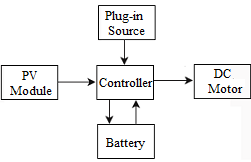
\includegraphics[width=\linewidth]{system_block.png}
		\caption{Block diagram of electric drive system of solar car}
		\label{fig:system_block}
	\end{figure}
	\subsection{Calculation of Solar irradiance}
	The model used to portray total solar irradiation on a solar panel, $G_{TP}$, considers direct solar beam on the panel $G_{BP}$, diffuse radiation $G_{DP}$, and ground reflected irradiance $G_{RP}$ \cite{deodusabe}. The general equation of $G_{TP}$ is given by,
	\begin{equation}
	\label{eq:gt}
	G_{TP} = G_{BP} + G_{DP} + G_{RP}
	\end{equation}
	\subsubsection{Direct solar beam radiation}
	If $G_B$ is the direct beam radiation at the surface of the earth and $\theta$ is the angle of incidence between the normal to the panel face and the incoming direct beam, the direct beam radiation $G_{BP}$ is given by,
	
	\begin{equation}
	\label{gbp}
	G_{BP}= G_Bcos\theta
	\end{equation}
	If $n$ is the day number (1-365) of the current day of a year, $G_B$ is calculated as, 
	\begin{equation}
	\label{gb}
	G_{B}= G_0exp\left(-\frac{K}{sine\beta}\right)
	\end{equation}
	where $G_0$ is the extraterrestrial radiation and $\beta$ is the altitude (zenith) angle of the sun, the angle between the sun and the local horizontal beneath the sun \cite{deodusabe}. They are determined by,
	\begin{equation}
	\label{g0}
	G_{0}= 1150+sin\frac{360\left(n-275\right)}{365}
	\end{equation}
	\begin{equation}
	\label{k}
	K= 0.174+0.035sin\frac{360\left(n-275\right)}{365}
	\end{equation}
	
	If the latitude of the region where the solar panel is placed is $L$, angle of declination is $\delta$ and the hour angle is $H$, $\beta$ can be found using the following equations,
	\begin{equation}
	\label{sinbeta}
	sin\beta= cosL cos\delta cosH+sinLsin\delta
	\end{equation}
	\begin{equation}
	\label{delta}
	\delta= 23.45sin\frac{360\left(284+n\right)}{365.25}
	\end{equation}
	\begin{equation}
	\label{h}
	H= \frac{15\degree}{hour}\left(\textit{hours before solar noon}\right)
	\end{equation}
	
	The “hours before solar noon” is positive before noon and
	negative after noon. $cos\theta$ of \eqref{gbp} is determined by \eqref{costheta} where ${\varphi}$ is the slope of the panel, ${\phi}_P$ is the azimuth of the panel.
	
	\begin{equation}
	\label{costheta}
	cos\theta = cos\beta cos\left({\phi}_S-{\phi}_P\right)sin\varphi+sin\beta cos\varphi
	\end{equation}
	
	The azimuth of the sun ${\phi}_S$ is given by,
	\begin{equation}
	\label{phis}
	{\phi}_S = sin^{-1}\frac{cos\delta sinH}{cos\beta}
	\end{equation}
	\subsubsection{Diffuse Radiation}
	The model of diffuse component of radiation on a flat
	solar panel is given by,
	\begin{equation}
	\label{gdp}
	G_{DP} = SG_B\frac{1+cos\varphi}{2}
	\end{equation}
	where the sky diffuse factor $S$ is computed as follows,
	\begin{equation}
	\label{S}
	S = 0.095+0.04sin\frac{360\left(n-100\right)}{365}
	\end{equation}
	
	\subsubsection{Reflected Radiation}
	The reflected radiation term on a surface of any direction is modeled as,
	\begin{equation}
	\label{grp}
	G_{RP}=\rho G_B\left(sin\beta + S\right)\frac{1-cos\varphi}{2}
	\end{equation}
	where $\rho$ is called the ground reactance or albedo; for concrete of the road, the value of it is estimated as 0.55 \cite{albedo}.
	
	\subsection{Electrical Model of Solar Panel}
	A solar cell is the unit component of a solar module. When there is no sunlight, a solar cell is not an active device; it works as a diode. If it is connected to an external supply it generates a current $I_D$, called diode current.
	\begin{figure}[!b]
		\centering
		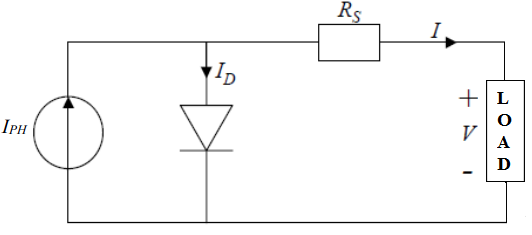
\includegraphics[width=\linewidth]{cell_electric.png}
		\caption{Electric equivalent diagram of a solar cell.}
		\label{fig:solarcell}
	\end{figure}
	That is why the electric circuit model of solar cell is like \figref{fig:solarcell}, which contains a current source $I_{PH}$, a diode and a series resistance $R_s$ representing the internal resistance of a cell. The net current $I$ is therefore the difference between $I_{PH}$ and $I_D$ as \eqref{eq:iph}.
	
	\begin{equation}
	\label{eq:iph}
	I = I_{PH}-I_D = I_{PH}-I_0\left[exp\left(\frac{V+IR_S}{V_t}\right)-1\right] 
	\end{equation}
	where $V$ is the voltage across the load. $I_0$ is the dark saturation current and it strongly depends on temperature \cite{lorenzo}. The thermal voltage of cell $V_t$ is calculated as \eqref{eq:vtc},
	
	\begin{equation}
	\label{eq:vtc}
	V_t = \frac{mkT_C}{q}
	\end{equation}
	where $m$ is idealising factor, $k$ is Boltzmann’s gas constant, $T_C$ is the absolute temperature of the cell, $e$ is electronic charge. $T_C$ depends on both the ambient temperature $T_a$ and irradiance $G_a$ as given by the following empirical relation,
	
	\begin{equation}
	\label{eq:tc}
	T_C = T_a + C_2G_a
	\end{equation}
	Where $C_2$ is a constant computed approximately as 0.03~Cm\textsuperscript{2}/W.
	
	An equation to calculate the series resistance of a cell is deduced as \eqref{eq:rsc0}. 
	
	\begin{equation}
	\label{eq:rsc0}
	R_S = \frac{V_{OC,0}}{I_{SC,0}}-\frac{\frac{\left(V_{OC,0}\right)^2}{V_{t,0}}-V_{OC,0}\ln\left(\frac{V_{OC,0}}{V_{t,0}}+0.72\right)}{P_{max,0}\left(\frac{V_{OC,0}}{V_{t,0}}+1\right)V_{OC,0}\left(I_{SC,0}\right)^2 } 
	\end{equation}
	
	Here, $V_{OC}$, $I_{SC}$ and $P_{max}$ are the open circuit voltage, short circuit current and maximum power respectively; the added subscript '0' indicates that the parameters are measured under standard temperature ($298K$) and irradiance ($1000 W/m^2$). The values of these parameters for standard condition are collected from the manufacturer's data-sheet.
	
	Cells are grouped in series or parallel or both to create module to supply higher current or voltage at the module terminal. A generalized figure of the module is shown in \figref{fig:module}, where $N_{PM}$ number of parallel branches and $N_{SM}$ number of series brunches are connected. 
	
	An equation for the module current $I_M$ having a voltage $V_M$ at its load terminals is derived in \cite{pvmodel} as \eqref{eq:IM} where the subscript 'M' indicates that the corresponding parameter belongs to an entire solar module.
	\begin{equation}
	\label{eq:IM}
	I_M = I_{SC,M}\left[1-exp\left(\frac{V_M-V_{OC,M}+R_{S,M}I_M}{N_{SM}V_{t,M}}\right)\right] 
	\end{equation}
	
	The parameters $I_{SC,M}$, $V_{OC,M}$, $R_{S,M}$ and $V_{t,M}$ of a module having $N_{SM}$ number of series branches and $N_{PM}$ number of parallel branches can be calculated using the following equations,
	
	\begin{equation}
	\label{eq:iscm}
	I_{SC,M}=I_{SC} N_{PM}
	\end{equation}
	
	\begin{equation}
	\label{eq:vocm}
	V_{OC,M}=V_{OC} N_{SM}
	\end{equation}
	
	\begin{equation}
	\label{eq:rsm}
	R_{S,M}=R_S \frac{N_{SM}}{N_{PM}}
	\end{equation}
	
	\begin{equation}
	\label{eq:vtm}
	V_{t,M} = V_tN_{SM}
	\end{equation}
	
	The short circuit current basically proportional to the irradiance of the sun $G_a$ as,
	
	\begin{equation}
	\label{eq:isc}
	I_{SC} = C_1G_a 
	\end{equation}
	
	Here $C_1$ is a constant defined by \eqref{eq:c1}. $G_a$ is the irradiance of the sun on the surface of the earth and $G_{a,0}$ is the standard irradiance($1000 W/m^2$).
	
	\begin{equation}
	\label{eq:c1}
	C_1 = \frac{I_{SC,0}}{G_{a,0} }
	\end{equation}
	
	The open circuit voltage of the cell depends on the temperature of the solar cells as,
	
	\begin{equation}
	\label{eq:voc}
	V_{OC} = V_{OC,0} + C_3\left(T_C-T_0\right)
	\end{equation}
	
	The constant $C_3$ is usually considered to be $-2.3~mV/C$ \cite{pvmodel} and $T_0$ is the standard temperature ($298K$).
	
	
	\begin{figure}[!tb]
		\centering
		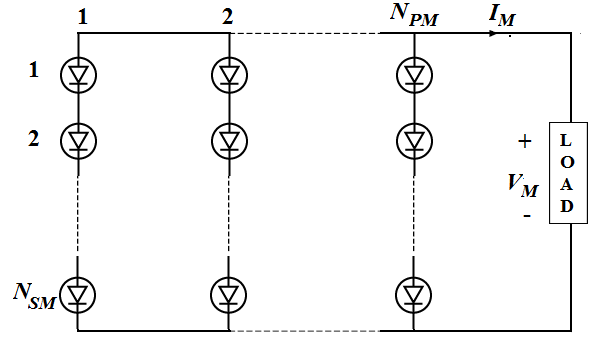
\includegraphics[width=\linewidth]{cell_array.png}
		\caption{Photovoltaic cells in series and parallel in a photovoltaic module}
		\label{fig:module}
	\end{figure}
	
	
	\subsection{Modeling of Battery}
	\begin{figure}[!b]
		\centering
		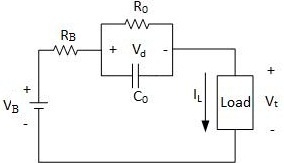
\includegraphics[width=0.7\linewidth]{Thevenin.jpg}
		\caption{Th\'{e}venin Battery Model}
		\label{fig:thevenin}
	\end{figure}
	
	The model used for battery is based on Th\'{e}venin battery model \cite{bat_thevenin} as shown in  \figref{fig:thevenin}, where $R_0$ and $C_0$ are the resistance and capacitance between electrodes of the battery, $R_B$ is the series resistance, $V_B$ is the open circuit voltage and $I_L$ is the load current. All of the three parameters namely  $V_B$, $R_B$ and $V_d$ in \figref{fig:thevenin} are functions of $\mathit{SOC}$ and have been evaluated experimentally for our batteries \cite{sadia}.
	
	The load current, $I_L$  for a load which draws out Power $P$ can be calculated using \eqref{eq:IL} as in \cite{bat_thevenin}.
	\begin{equation}
	\label{eq:IL}
	I_L = \frac{\left(V_B-V_d\right)-\sqrt{\left(V_B-V_d\right)^2-4R_BP}}{2R_B} 
	\end{equation}
	
	In case, battery is being charged by $I_{CH}$ current, it flows opposite to $I_L$ and the overall current flowing through the battery is reduced to $(I_L-I_{CH})$.
	
	With $I_L$ known, the terminal voltage $V_t$ and the total charge dissipated from battery $Q_{dis}$ in time $t$ can be calculated as,
	
	\begin{equation}
	\label{eq:Vt}
	V_t = V_B-I_LR_B-V_d
	\end{equation}	
	
	\begin{equation}
	\label{eq:Qdis}
	Q_{dis}=I_Lt
	\end{equation}	
	The new $\mathit{SOC}$ of the battery after time $t$ is then given by,
	
	\begin{equation}
	\label{eq:SOCn}
	SOC\left(new\right) = SOC\left(old\right)-\frac{Q_{dis}}{C(T_a)}
	\end{equation}	
	where $C(T_a)$ is the capacity of the battery which also depends on the ambient temperature $T_a$. According to \cite{temp_cap}, a relationship between the battery capacity and the ambient temperature is derived as, using a linear fitting approximation,
	\begin{equation}
	\label{eq:temp_cap}
	C(T_a) = C_0(0.0082T_a-0.77)
	\end{equation}
	where $C_0$ is the discharge capacity at $25\degree C$.
	
	With the new $\mathit{SOC}$ calculated as in \eqref{eq:SOCn},  $V_B$, $R_B$ and $V_d$ are re-evaluated according to the following relations which were determined experimentally in \cite{sadia}.
	
	\begin{equation}
	V_B=1.4667\textit{SOC}+11.0233
	\end{equation}
	\begin{equation}
	V_d=0.086 \textit{SOC } - 0.011
	\end{equation}
	\begin{equation}
	R_B= -0.0531\textit{SOC} + 0.066
	\end{equation}
	
	
	\subsection{Power Calculation of DC Motor}
	Power required by the motor to drive the car can be estimated by adding together individual force components that arise from different physical effects. The major three forces are the force of acceleration $F_A$, aerodynamic drag force $F_D$, force exerted by the air against the movement of the car, and the frictional force $F_R$, force required to overcome the frictional resistance between the wheel and the road \cite{leitman}. Summing up, total driving force, $F_T$ is obtained as,
	
	\begin{equation}
	\label{eq:FT}
	F_T = F_{R}+F_{D}+F_{A}
	\end{equation}
	
	The car will have a force of acceleration only when it is accelerating, otherwise it will be zero when running at a constant velocity. All of the three major forces are calculated using the following equations,
	
	\begin{equation}
	\label{eq:Froll}
	F_{R} = \mu_Rmg
	\end{equation}
	\begin{equation}
	\label{eq:Fdrag}
	F_{D} = \frac{1}{2} C_D \rho A_{C\!R\!O\!S\!S} v^2
	\end{equation}
	\begin{equation}
	\label{eq:Facc}
	F_{A} = ma
	\end{equation}
	
	Here, $m$ is the mass, $A_{\mathit{CROSS}}$ is the frontal cross sectional area, $v$ is the velocity, $a$ is the acceleration of the car, $\rho$ is the air mass density, $C_D$ is the coefficient of aerodynamic drag force,  $g$ is the gravitational acceleration, and $\mu_R$ is the coefficient of rolling resistance.
	
	If the car is running at a velocity of $v$ then the power exerted by the shaft of the motor can be expressed as,
	\begin{equation}
	\label{eq:PT}
	P_{T} = F_T v.
	\end{equation}
	
	If the efficiency of the motor is $\eta_{m}$, the power required to be supplied by the battery to the motor is given by,
	
	\begin{equation}
	\label{eq:Preq}
	P = \frac{P_T}{\eta_{m}}
	\end{equation}
	
	\subsection{Mechanism of charge controller}
	There are four set points in a charge controller, two to avoid overcharge and two for overdischarge as in \cite{leitman}. The maximum 
	SOC the batteries are allowed to reach and above which solar panels are disconnected from the battery is array disconnect SOC (ADS). Then the battery may discharge to a SOC level low enough to start charging again; the level is array reconnect SOC (ARS). Similarly, the load is disconnected at the minimum SOC, namely low SOC load disconnect (LSD), after which more discharging may damage the battery. Then the battery may charge for some time, the SOC rises and the load is connected again at a level of load reconnect SOC (LRS). The points are depicted in \figref{fig:setpoints} 
	
	\begin{figure}[!tb]
		\centering
		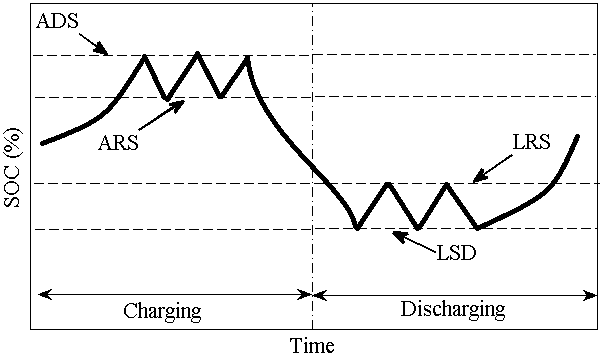
\includegraphics[width=\linewidth]{charge_controller_mech.png}
		\caption{Charge Controller set points}
		\label{fig:setpoints}
	\end{figure}
	
	\section{Implementation in Simulink}
	The implementation of the aforementioned models of solar panel, battery, motor power and charge controller are described in the following subsections.
	\subsection{Implementation of solar panel}
	The aforementioned algorithm of calculating module current is implemented in the graphical programming language of Simulink where the inputs are ambient temperature $T_a$, solar irradiance $G_a$ and the terminal voltage  of the load $V_t$, and it gives $I_{CH}$ as output as \figref{fig:panelmask} shows. The algebraic constrain block the figure is used to solve the nonlinear equation of \eqref{eq:IM}. The numbers of different equations used in the model of are imprinted on the corresponding function blocks.
	\begin{figure}[!tb]
		\centering
		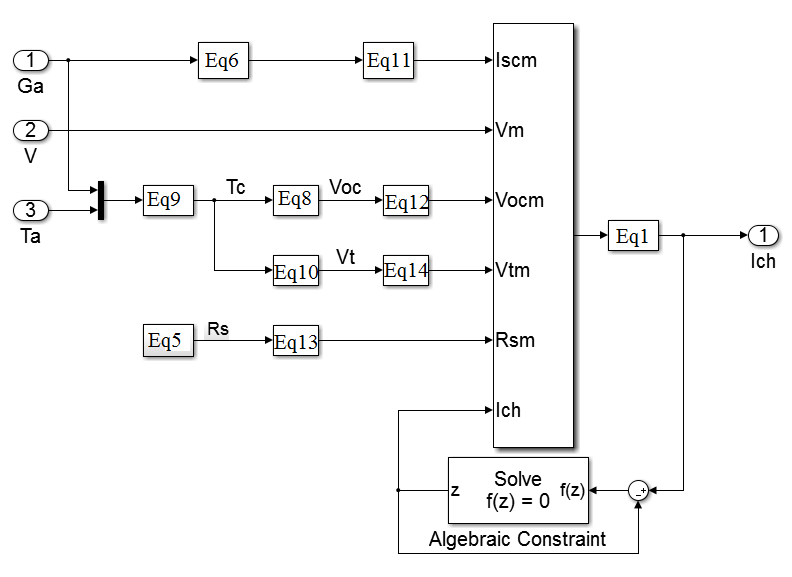
\includegraphics[width=\linewidth]{panel_model.png}
		\caption{Inside view of the mask of the PV module model}
		\label{fig:panelmask}
	\end{figure}
	\subsection{Implementation of Battery Model}
	\figref{fig:batterymask} shows the battery model in Simulink where the power required $P$ and charging current $I_{CH}$ are the inputs to battery. It calculates $I_L$, $V_t$ and SOC after dissipating power for a certain time and gives out as outputs. Eq(1), Eq(2) etc. labeled in the diagram refer to the corresponding equation numbers in this paper. The time interval after which the model calculates dissipated charge and records a new SOC can be fixed by the mask parameter dialog box along with the nominal capacity of the battery, initial state of charge, temperature and the number of batteries in series.
	\begin{figure}[!tb]
		\centering
		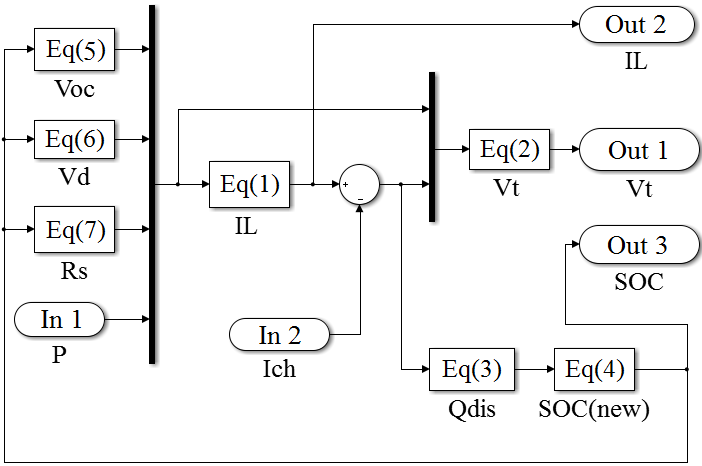
\includegraphics[width=\linewidth]{battery_model.png}
		\caption{Implementation of Battery model in Simulink}
		\label{fig:batterymask}
	\end{figure}
	\subsection{Implementing Load Block in Simulink}
	The Simulink block of Load, named ‘Load’ in \figref{fig:solarcar}, takes inputs of variable velocity on different time frames and some invariants related to the car e.g. its weight, frontal area. If the car moves at velocity $v_1$ kilometer per hour (kph) for $t_1$ minutes, comes to a halt and rests for $t_1^r$  minutes, and then starts again at $v_2$  kph at which it runs for another $t_2$ minutes, the input format is $v=[v_1    0    v_2 ]$ and $t=[t_1     t_1^r     t_2 ]$. Time $t_1$  consists of the time at which the car accelerates from static position to reach $v_1$, the time it runs at constant $v_1$  kph, and fall time when the car decelerates to halt. The inputs are transferred to a MATLAB program which gives a timeseries variable $P$ using the equations \eqref{eq:FT} to \eqref{eq:Preq}. The signal building block of load has some presets e.g. Busy road, Highway, Empty road etc. to select easily some preloaded values of the variables or the users may produce a set of value according to their concern.
	
	\subsection{Implementation of Charge Controller}
	\figref{fig:chargemask} implements the charge controller in SIMULINK. There are two ‘if’ blocks in the diagram; upper one is controlling the discharging state and lower one the charging state. If the SOC goes below the given level to turn off discharging, and the discharging process is not switched off yet, the upper if block commands the Discharge off block to disconnect the load. On the other hand, if the SOC is high enough to turn on discharging, the same if block triggers Discharge on action block to connect the load and deliver input power to the output. Same mechanism applies for the charging state controller ‘if’ block except, this time, the input charging current flows to output when charging is turned on.
	\begin{figure}[!tb]
		\centering
		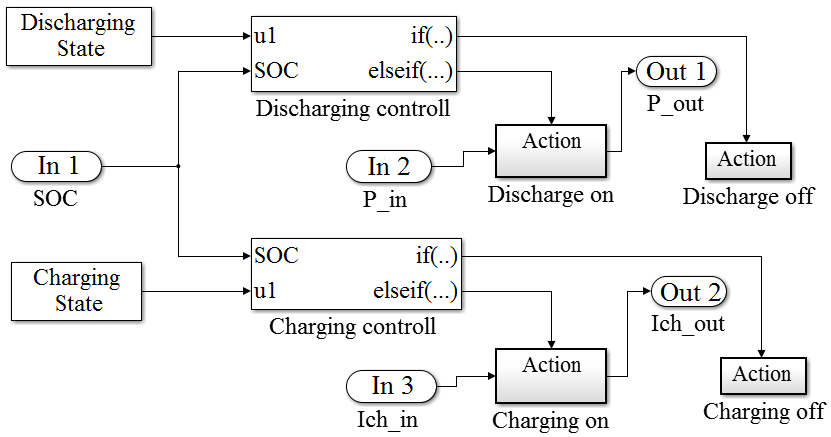
\includegraphics[width=\linewidth]{charge_controller.png}
		\caption{Implementation of charge controller model in Simulink}
		\label{fig:chargemask}
	\end{figure}
	
	\subsection{Combining the Components}
	All the components portrayed in earlier sections are packed inside subsystems and combined together to build a complete model of vehicle as in \figref{fig:solarcar}. All data found by the simulation are transfered to the MATLAB workspace to plot and analyze the results.
	
	\begin{figure}[!tb]
		\centering
		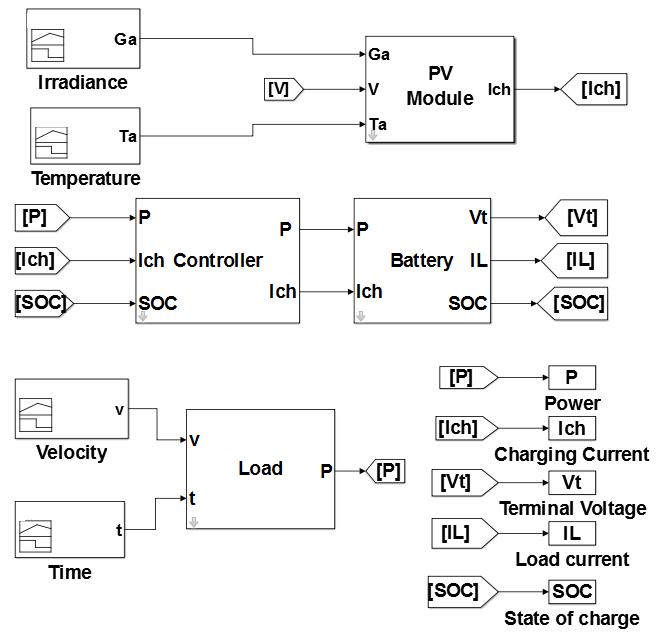
\includegraphics[width=\linewidth]{solar_car.png}
		\caption{The model of the solar car combining all individual components}
		\label{fig:solarcar}
	\end{figure}
	
	\section{Results and Discussions}
	An itinerary is assumed for a Dhaka city dweller from his home to office, which is 18 km long. For the sake of convenience, it is assumed that the person leaves his home in the morning with his car fully charged and reaches his office by driving 10\% of the distance at 10 kilometer per hour (kph) and rest of the road either 30 kph or 60 kph depending on the road condition. In the afternoon, he returns by the same route with same speed characteristics.
	
	\subsection{Performance Analysis}
	
	
	\begin{figure}[!tb]
		\centering
		\includegraphics[width=\linewidth]{power_vel_curve.png}
		\caption{Variation in (a) car speed, and (b) motor power of the battery during one full trip as the car travels from origin to its destination.}
		\label{fig:powercurve}
	\end{figure}
	\begin{figure}[!tb]
		\centering
		\includegraphics[width=\linewidth]{car_speed.png}
		\caption{Variation in SOC in spring with the car traveling (a) 90\%, (b) 60\%, and (c) 30\% of the road at the top speed. Plot (d) is that for 30\% with 20 number of stoppages.}
		\label{fig:car_speed}
	\end{figure}
	\figref{fig:powercurve} shows the plots of power required $P$ and car speed $v$ as the car travels at different velocities from its origin to destination. The top most plot shows the different velocities of the car during its trip which starts with 10 kph at its origin covering 5\% of the distance, goes at after that for 15\% of the road, then goes at 60 kph for 60\% of the road, after which it goes at 30 kph and 10 kph for the rest of 15 and 5 of the road, respectively, before it reaches the destination. For the sake of simplicity we assumed a constant acceleration with which the car reaches the maximum speed from its rest position and a constant deceleration with which it comes to a halt from its maximum speed. For higher speed higher acceleration and deceleration are assumed than those at lower speed. The required power increases gradually with the increase in car speed as can be seen from the power plot below the velocity plot in \figref{fig:powercurve}. The power drops abruptly whenever the velocity reaches target speed because the driver releases the accelerator at that time, and hence force of acceleration becomes zero requiring less power to drive.
	\begin{table}[!t]
		\renewcommand{\arraystretch}{1.3}
		\caption{Properties of solar car}
		\label{bat_table}
		\centering
		\begin{tabular}{|C{.265\columnwidth}|C{.505\columnwidth}|C{.08\columnwidth}| }
			\hline
			\centering
			\textbf{Components} & \textbf{Parameters} & \textbf{Value} \\ \hline
		\end{tabular}
		\begin{tabular}{|p{2.35cm}|c|c|}
			\multirow{3}{*}{\textbf{Panel\cite{srea}}}
			& \multicolumn{1}{L{.5\columnwidth}|}{Maximum Power, $P_{max}$ (W)} & \multicolumn{1}{c|}{50} \\\cline{2-3}
			& \multicolumn{1}{l|}{Open circuit voltage, $V_{OC}$ (V)} & \multicolumn{1}{c|}{18} \\\cline{2-3}
			& \multicolumn{1}{l|}{Short circuit current, $I_{SC}$ (A)} & \multicolumn{1}{c|}{3.11} \\\hline
			
			\multirow{2}{*}{\textbf{Battery\cite{sadia}}}
			& \multicolumn{1}{L{.5\columnwidth}|}{Capacity of a battery, $C$ (Ah)} & \multicolumn{1}{c|}{70} \\\cline{2-3}
			& \multicolumn{1}{l|}{Number of batteries in series, $N$ } & \multicolumn{1}{C{0.7cm}|}{5} \\\hline
			
			\multirow{4}{*}{\textbf{Charge controller}}
			& \multicolumn{1}{L{.5\columnwidth}|}{Array disconnect SOC, \textit{ADS(\%)}} & \multicolumn{1}{c|}{100} \\\cline{2-3}
			& \multicolumn{1}{L{.5\columnwidth}|}{Array reconnect SOC, \textit{ARS(\%)} } & \multicolumn{1}{c|}{85} \\\cline{2-3}
			& \multicolumn{1}{L{.5\columnwidth}|}{Low SOC load disconnect, \textit{LSD (\%)}} & \multicolumn{1}{c|}{25} \\\cline{2-3}
			& \multicolumn{1}{l|}{Load reconnect SOC, \textit{LRS(\%)}} & \multicolumn{1}{c|}{50} \\\hline
			
			\multirow{4}{*}{\textbf{Vehicle platform\cite{srea}}}
			& \multicolumn{1}{L{.5\columnwidth}|}{Mass of the car, $m$ (kg)} & \multicolumn{1}{c|}{500} \\\cline{2-3}
			& \multicolumn{1}{L{.5\columnwidth}|}{Maximum velocity, $v_{max}$ (kph)} & \multicolumn{1}{c|}{60} \\\cline{2-3}
			& \multicolumn{1}{L{.5\columnwidth}|}{Time to reach max. velocity, $t_{max}$ (min)} & \multicolumn{1}{c|}{1.5} \\\cline{2-3}
			& \multicolumn{1}{l|}{Frontal area, $A_\mathit{CROSS}$ ($m^2$)} & \multicolumn{1}{c|}{1.1} \\\hline
			
			\multirow{3}{*}{\textbf{Environment\cite{leitman}}}
			& \multicolumn{1}{L{.5\columnwidth}|}{Coeff. of rolling resistance, $\mu_{R}$ (W)} & \multicolumn{1}{c|}{0.025} \\\cline{2-3}
			& \multicolumn{1}{l|}{Coeff. of aerodynamic drag force, $C_D$} & \multicolumn{1}{c|}{0.035} \\\cline{2-3}
			& \multicolumn{1}{l|}{Air density, $\rho (kg/m^3)$} & \multicolumn{1}{c|}{3.11} \\\hline
		\end{tabular}
	\end{table}
	
	\figref{fig:car_speed} shows how the SOC varies when the car moves at the top speed of 60 kph for different lengths of the road. As can be seen from this figure, SOC drops to almost 67\% when the car runs 90\% of the road at the top speed, indicating about 13\% additionally required charge at this speed. However, SOC drops to only 78\% when the car runs only 30\% of the road at the top speed with 60\% at half the top speed and the rest 10\% at 10 kph, indicating more that 40\% reduction in energy consumption at this slower speed and almost no necessitiy of additional charge. The higher energy requirement at higher speed is due to the higher aerodynamic drag force which increases as the square of the velocity according to \eqref{eq:Fdrag}. Energy requirement is further reduced if the trip is accompanied with frequent breaks (topmost plot in \figref{fig:car_speed}) during heavy traffic congestion which is a common phenomena in the city of Dhaka.
	
	\begin{figure}[!tb]
		\centering
		\includegraphics[width=\linewidth]{SOC_seasons.png}
		\caption{Variation of SOC in (a) cloudy summer, (b) winter, (c) spring, and (d) summer throughout a day with the car traveling at 60\% of the road at top speed.}
		\label{fig:SOCseasons}
	\end{figure}
	\begin{figure}[!tb]
		\centering
		\includegraphics[width=\linewidth]{Withmass.png}
		\caption{Variation of SOC for a car with mass (a) 1000kg, (b) 800 kg and (c) 500 kg with the car traveling 60\% of the time at top speed in summer.}
		\label{fig:mass}
	\end{figure}
	
	\figref{fig:SOCseasons} shows how the SOC varies when the car travels at the speed described earlier in different seasons of the year. The car can not only travel solely on solar power during summer seasons but also store some more energy at the end of the day. However, in spring and winter some additional energy will be required. However, if the car mass increases, the required energy will also be increased. If the mass of the car doubled from 500kg to 1000kg, the SOC in the end of the day decreases by 25\% as in \figref{fig:withmass}.
	
	\subsection{Environmental Impact}
	While there are no global warming emissions associated with generating electricity from solar energy, there are emissions associated with other stages of the solar life-cycle, including manufacturing, materials transportation, installation, maintenance, and decommissioning and dismantlement. Most estimates of life-cycle emissions for photovoltaic systems are between 26 and 60 grams of carbon dioxide equivalent per kilowatt-hour (\ce{CO2}eq/kWh) \cite{greenhous}.
	
	\begin{figure}[!b]
		\centering
		\includegraphics[width=\linewidth]{Additional4.png}
		\caption{Additional energy required by the car throughout a year with the car moving at 60\% of the road at top speed with 10 number of stoppages.}
		\label{fig:additionalenv}
	\end{figure}
	
	\begin{figure}[!b]
		\centering
		\includegraphics[width=\linewidth]{Additional2.png}
		\caption{Emission of \ce{CO2}eq gas for every month with a mass of 500 kg, 800 kg and 1000 kg with the car moving 60\% of the road at top speed}
		\label{fig:withmass}
	\end{figure}
	
	In addition to that, the proposed solar car needs different amount of additional energy to be supplied from national grid in seasons other than summer. In \figref{fig:additionalenv} the bars represent the average amount of energy supplied by the solar panels in a day for each month of a year while the car travels 30\% of the road at top speed. The gap between the top of a bar and the dashed line of required energy is the measure of energy drawn from national grid. Apart from April and May, where the supplied energy is in excess of what required, the additional energy differs from month to month depending on the sun's position and the cloud factor of that month. The term cloud factor stands for the ratio of solar irradiance available on the surface of a solar panel to the ideal irradiance if the sky is clear. In January, for instance, about 60\% of ideal irradiance falls on a solar panel due to excessive fog, but in April a panel can get excess to almost 80\% and hence, the respective cloud factor of January and April is 0.6 and 0.8. Considering this factor a more pragmatic estimation of additional energy is calculated for each month having 25 working days. The total additional energy for an entire year is found by summing up the data of each month is around 55 kWh.
	
	
	
	Generally, the electricity of national grid is produced by fuel driven power plants emitting a considerable amount of carbon dioxide which should also be attributed to the solar car while computing its environmental impact. The grid electricity emission factor is taken as 0.637 kg-\ce{CO2}eq/kWh \cite{gridemission}. \figref{fig:withmass} shows the average emission of \ce{CO2}eq gas in grams in a day for each month of a year. The effect of varying weight of the car on the greenhouse gas emission is also depicted in the figure. The total amount of \ce{CO2}eq gas emission over a year for a 500 kg car is 34 kg and for a 1000 kg car 134 kg.
	
	\begin{table}[!t]
		\centering
		\caption{Life Cycle Cost Analysis of a Solar Car}
		\label{costtable}
		\begin{tabular}{|l|c|c|c|c|}
			\hline
			\multicolumn{1}{|c|}{\textbf{Component}} & \textbf{\begin{tabular}[c]{@{}c@{}}Number\\ of Units\end{tabular}} & \textbf{\begin{tabular}[c]{@{}c@{}}Unit\\ Cost\\ (BDT)\end{tabular}} & \textbf{\begin{tabular}[c]{@{}c@{}}Initial\\ Cost\\ (BDT)\end{tabular}} & \textbf{\begin{tabular}[c]{@{}c@{}}Present\\ Worth\\ (BDT)\end{tabular}} \\ \hline
			Solar panel & 250W & \begin{tabular}[c]{@{}c@{}}140 per\\ Watt\end{tabular} & 35,000 & 35,000 \\ \hline
			Battery & 5 & 7,500 & 37,500 & 37,500 \\ \hline
			\begin{tabular}[c]{@{}l@{}}Battery 5 Yrs\\ Battery 10 Yrs\\ Battery 15 Yrs\\Battery 20 years\end{tabular} & \begin{tabular}[c]{@{}c@{}}5\\ 5\\ 5\\5\end{tabular} &  & \begin{tabular}[c]{@{}c@{}}37,500\\ 37,500\\ 37,500\\ 37,500\end{tabular} & \begin{tabular}[c]{@{}c@{}}36,360\\ 34,183\\ 31,160\\ 27,541\end{tabular} \\ \hline
			\begin{tabular}[c]{@{}l@{}}Charge Controller\end{tabular} & 1 & 25,000 & 25,000 & 25,000 \\ \hline
			
			\begin{tabular}[c]{@{}l@{}}Charge Controller 10 Yrs\\ Charge Controller 20 years\end{tabular} & \begin{tabular}[c]{@{}c@{}}1\\ 1\end{tabular} &  & \begin{tabular}[c]{@{}c@{}} 25,000 \\ 25,000 \end{tabular} & \begin{tabular}[c]{@{}c@{}} 23,503
				\\ 22,096 \end{tabular}\\ \hline
			
			DC motor & 1 & 40,000 & 40,000 & 40,000 \\ \hline
			\begin{tabular}[c]{@{}l@{}}DC motor 10 Yrs\\ DC motor 20 years\end{tabular} & \begin{tabular}[c]{@{}c@{}}1\\ 1\end{tabular} &  & \begin{tabular}[c]{@{}c@{}} 40,000 \\ 40,605 \end{tabular} & \begin{tabular}[c]{@{}c@{}} 37,605 \\ 35,354 \end{tabular}\\ \hline
			
			\begin{tabular}[c]{@{}l@{}}National grid utility bill\end{tabular} &  &  & 620 & 14,407 \\ \hline
			
			\begin{tabular}[c]{@{}l@{}}Annual Maintenance\end{tabular} &  &  & 2,000 & 37,740 \\ \hline
			
			
			Life Cycle Cost & \multicolumn{4}{r|}{437,050} \\ \hline
		\end{tabular}
	\end{table}
	
	\begin{table*}[t]
		\centering
		\caption{Operation Cost Analysis of a Fuel-Based Car}
		\label{opcost}
		\begin{tabular}{|l|c|c|c|c|}
			\hline
			\multicolumn{1}{|c|}{\multirow{2}{*}{\textbf{Component}}} & \multicolumn{2}{c|}{\textbf{First year (BDT)}} & \multicolumn{2}{c|}{\textbf{Present worth for 25 years (BDT)}} \\ \cline{2-5} 
			\multicolumn{1}{|c|}{} & \textbf{\begin{tabular}[c]{@{}c@{}}Without traffic\\ congestion\end{tabular}} & \textbf{\begin{tabular}[c]{@{}c@{}}With traffic \\ congestion\end{tabular}} & \textbf{\begin{tabular}[c]{@{}c@{}}Without traffic\\ congestion\end{tabular}} & \textbf{\begin{tabular}[c]{@{}c@{}}With traffic\\ Congestion\end{tabular}} \\ \hline
			Fuel & 55,870 & 89,185 & 12,98,312 & 20,72,491 \\ \hline
			\begin{tabular}[c]{@{}l@{}}Annual Maintenance\\     \hspace{0.5cm}   Engine Oil, Filter Replacement\\  \hspace{0.5cm}      Servicing, Fitness Test, Tax\end{tabular} & \multicolumn{2}{c|}{\begin{tabular}[c]{@{}c@{}}\\30,000\\ 18,000\end{tabular}} & \multicolumn{2}{c|}{\begin{tabular}[c]{@{}c@{}}\\697,142\\ 418,285\end{tabular}} \\ \hline
			Total Operation Cost & \multicolumn{2}{c|}{} &  1,995,454 & 2,490,777 \\ \hline
		\end{tabular}
	\end{table*}
	On the other hand, petrol produces 2.7 kilograms of greenhouse gas emissions per
	liter combusted \cite{iran}.
	
	When it comes to calculating how a fuel driven car affects the atmosphere, the result is highly alarming. To travel from Uttara to Motijheel, a fuel driven car may burn 2 to 6 liters of petrol depending on the traffic condition and the type of the engine of the car. According to \cite{iran} petrol produces 2.7 kilograms of greehous gas per liter combusted leading to an emission of 11 kilogram of  \ce{CO2}eq gas to the atmosphere per day if an average of 4 liters of petrol is assumed for the trip. The harm a fuel driven car does to the environment in a week is higher than that of a solar car in an entire year.
	
	Apart from their feature of pollution free drive, the feature of solar car of requiring less energy at slower speed will be a big advantage over the fuel driven cars which consume more fuel at slower speed to cover the same distance due to inefficient burning of the fuel. Furthermore, fuel driven cars will keep buring fuel thus producing more pollution whenever in traffic congestion or waiting at a traffic signal, while the solar car, instead of consuming energy, will harness energy from the sun.
	
	\subsection{Economic Aspects}
	
	
	Life cycle cost (LCC) analysis is a way to determine the economic impact
	of current and future costs comprised of the
	cost of operating an item over its entire lifetime, starting from the time of initial acquisition till purchases made later \cite{messenger}.
	
	The LCC of the solar car includes the cost of the solar panel and the expenses related to the operation and the maintenance of the panel and the battery. Solar panels are expected to serve for no less than 25 to 30 years without requiring any major replacement. It is considered that with cautious taking care of, monocrystalline panels may even last till 40 years \cite{celik}. The initial cost of setting up a panel is quite high, but this investment is compensated by its long life of 25 to 30 years. Electric lead-acid batteries also have a high life cycle of 5 years and therefore will not require frequent replacements \cite{celik}. Manufactured three
	stage charge controllers usually have a factory warranty of 5
	years, but they have an expected lifetime of 15 years \cite{ecodirect}.
	Brushless DC Motors usually have a life span of more than 10000 hours that corresponds roughly to 10 years of operation with a car with a maximum of 4 hours of daily usage \cite{minebea}.
	
	
	
	In order to find the LCC, the present worth (PW) of all the components needs to be determined and then summed. Present worth of any item is the amount of money that needs to be invested at the present time in order to purchase the item 'n' years later, assuming an inflation rate of 100i\% and an interest or discount rate of 100d\%, and is given by,
	\begin{equation}
	\label{presentworth}
	PW = \left(\frac{1+i}{1+d}\right)^n \times C_0
	\end{equation}
	where $C_0$ is the initial cost of the item at the time of investment\cite{roger};
	
	For recurring expenses, which adds up to the total cost every year of operation, the individual PW of each element in the series can be added up to find the cumulative PW. Thus expenses such as the fuel cost and maintenance cost can be calculated using the following equation \cite{roger},
	\begin{equation}
	\label{realpw}
	PW = \frac{1-x^n}{1-x}C_0
	\end{equation}
	where
	\begin{equation}
	\label{x}
	x = \frac{1+i}{1+d}
	\end{equation}
	The values of the average inflation and interest rates of
	Bangladesh have been found to be 6.59\% and 7.25\%,
	respectively.
	
	
	We can further add the cost of electricity when the solar car will also be powered through main line electric supply during days of insufficient solar energy. The tariff of electricity supplied by Dhaka Electric Supply Company (DESCO) to home and business consumers with an average consumption over 400 units is BDT 11.25 per kWh of usage for residential use \cite{desco}. For 55 kWh calculated in the previous subsection the cost is BDT 620 a year, and BDT 15,500 for 25 years.
	
	
	Considering the costs of each component and their corresponding life span, the LCC of a solar car is found BDT 190,000 over a period of 25 years, considering 280 days of office commuting \cite{solar_car}.
	
	
	On the other hand, A 1500 cc car (e.g. Toyota Corolla X) which runs on gasoline on the streets of Dhaka can cover a maximum distance of about 17.24 km per liter without encountering any traffic congestions. If, however, there
	are heavy traffic jams on the road, the distance traveled per liter is reduced to a maximum of 10.8 km \cite{toyota}. Thus, the amount of petrol required to travel a distance of 40km for 280 days of a year are 1050 and 650 liters with and without traffic congestion respectively.According to the current price chart \cite{petrol}, the price of petrol is BDT 86 per liter, and hence BDT 2,305,500 with traffic congestion and BDT 1,445,500 without traffic congestion are the estimated cost of operating the car for a period of 25 years including other maintenance cost of the car as shown in Table \ref{opcost}. These figures, compared to that of a solar car, are shockingly high. 
	
	On top of the value calculated, costs in terms of environmental and health hazards also needs to be taken into account. It can be clearly seen the long run cost of running a fuel-based car far exceeds the cost of using and maintaining a solar car, both quantitatively and qualitatively.
	\section{Conclusion}
	Battery performance of a propsed solar car has been investigated while the car makes a trip from home to workplace of an office commuter under different road conditions, using a model developed in Matlab Simulink. It has been observed that energy requirement decreases significantly when the car runs at a slower speed due to lower air drag force at lower velocity. Thus for a city like Dhaka, where traffic congestion is a daily occurrence, solar car will be a perfect mode of transportation as it is not only emission free but also consumes less energy under heavy traffic congestion, unlike the fuel driven cars which consumes more energy and emit more toxic gases under such condition. 
	
	\bibliographystyle{IEEEtran}
	\bibliography{IEEEabrv,mySCarRef}
	
\end{document}

